\documentclass[a4paper]{article}
\usepackage[a4paper,  fancysections,  titlepage]{pdfEPUSP}
\usepackage[brazilian]{babel}
\usepackage[hidelinks]{hyperref}
\usepackage[alf]{abntex2cite}
\usepackage{tcolorbox}
\usepackage[hypcap=false]{caption}
\usepackage{amsmath, amssymb}
\usepackage{placeins}

\usepackage{minted}
\setminted{
autogobble,
baselinestretch=0.9,
encoding=utf8,
fontsize=\footnotesize,
python3=true,
style=vs,
}

\author{
\begin{align*}
    &\text{Gabriel Pereira de Carvalho} \qquad &\text{NUSP: 11257668} \\
    &\text{Lucas Xavier de Morais} \qquad &\text{NUSP: 18066592} \\
    &\text{Joaquin Lorenzo Pereira Condori} \qquad &\text{NUSP: 11857963}
\end{align*}
}
\date{}
\title{PSI5723: Introdução ao Projeto de Sistemas VLSI em CMOS}
\subtitle{Lista de Exercícios 2}

\begin{document}

\maketitle

\tableofcontents
\newpage

\section{Atrasos com aplicação de skew para porta NAND}

\subsection{Circuito de teste e aplicação do skew}

Nosso ponto de partida para a lista 2 foi a porta NAND implementada na lista 1, onde realizamos o layout, DRC, LVS e extração de capacitâncias parasitas. Esse modelo final foi o que utilizamos no circuito de teste, mostrado na Figura \ref{fig:nand-skew-config}, para os experimentos que vamos detalhar na sequência.

\begin{figure}[!htbp]
    \centering
    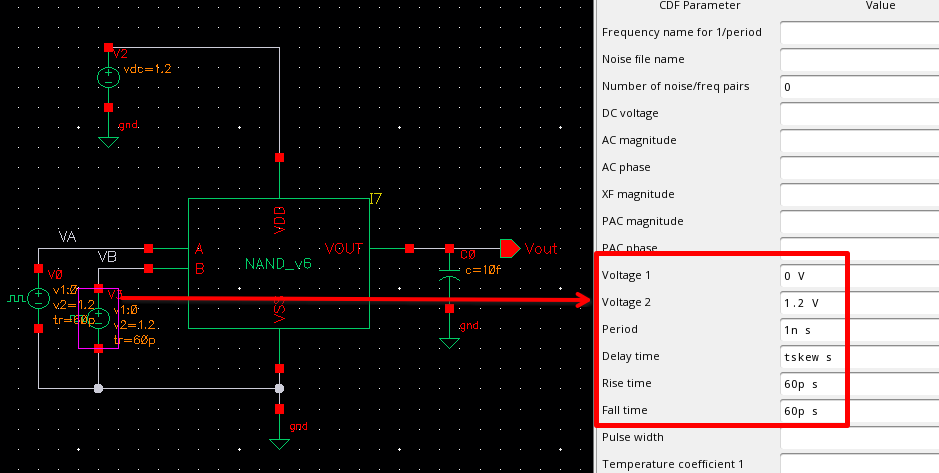
\includegraphics[width=0.95\linewidth]{imagens_lista2_NAND/NAND_tskew_dealy_configuration.png}
    \caption{Circuito de teste da NAND e parâmetros da fonte pulsada: alimentação de $1{,}2\,\mathrm{V}$, carga de $10\,\mathrm{fF}$, período de $1\,\mathrm{ns}$ e rampas de $60\,\mathrm{ps}$.}
    \label{fig:nand-skew-config}
\end{figure}

Assim como no setup da lista 1, as fontes são componentes \texttt{v\_pulse} da biblioteca \texttt{analogLib} que variam entre $0$ e $1{,}2\,\mathrm{V}$, com tempos de subida e de descida de $60\,\mathrm{ps}$ e período de $1\,\mathrm{ns}$. Os $200\,\mathrm{ps}$ solicitados são especificados como largura do pulso noo campo \textit{Pulse width}.

Para interpretar a varredura, adota-se
\begin{equation}
    t_{\mathrm{skew}} = t_B - t_A.
    \label{eq:nand-skew-definicao}
\end{equation}

Assim, $B$ antecede $A$ para skew negativo e sucede $A$ para skew positivo; em zero, as entradas comutam simultaneamente. Para evitar que tempos negativos durante a varredura da variável \texttt{tskew} utilizamos um atraso comum $t_0$ para $A$ e $t_0+t_{\mathrm{skew}}$ para $B$, com $t_0\geq200\,\mathrm{ps}$, o que é suficiente para evitar atrasos absolutos negativos.

A Figura~\ref{fig:nand-skew-varredura} mostra a varredura de $-200$ a $+200\,\mathrm{ps}$ em incrementos de $5\,\mathrm{ps}$, totalizando 81 pontos, realizada na ferramenta \textit{Parametric Analysis} do Virtuoso.

\begin{figure}[!htbp]
    \centering
    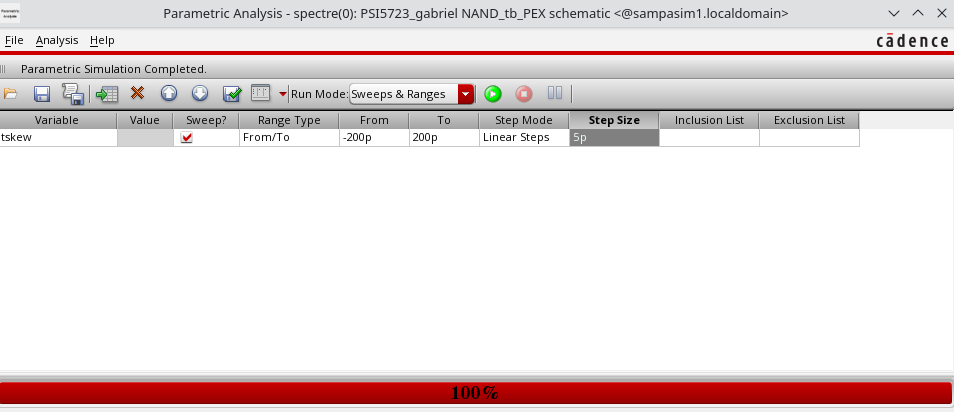
\includegraphics[width=\linewidth]{imagens_lista2_NAND/NAND_tskew_parameter_sweep_configuration.png}
    \caption{Varredura paramétrica da NAND entre $-200$ e $+200\,\mathrm{ps}$, com passo de $5\,\mathrm{ps}$.}
    \label{fig:nand-skew-varredura}
\end{figure}

\subsection{Critério de medição e índices das bordas}

As Figuras~\ref{fig:nand-skew-expr-lh} e~\ref{fig:nand-skew-expr-hl} apresentam as expressões usadas para os atrasos. Ambas selecionam a entrada \texttt{/VA}, correspondente a $A$, e a saída \texttt{/Vout}, com limiares de $0{,}6\,\mathrm{V}$, equivalentes a $50\%$ de $V_{DD}$. Foi selecionada a terceira ocorrência de cada borda, indicada por \texttt{nth1=3} e \texttt{nth2=3} assim como fizemos na lista 1, para evitar que condições iniciais da simulação afetem de alguma forma os valores medidos.

A Tabela~\ref{tab:nand-skew-medicao} reproduz os campos principais em formato legível.

\begin{figure}[!htbp]
    \centering
    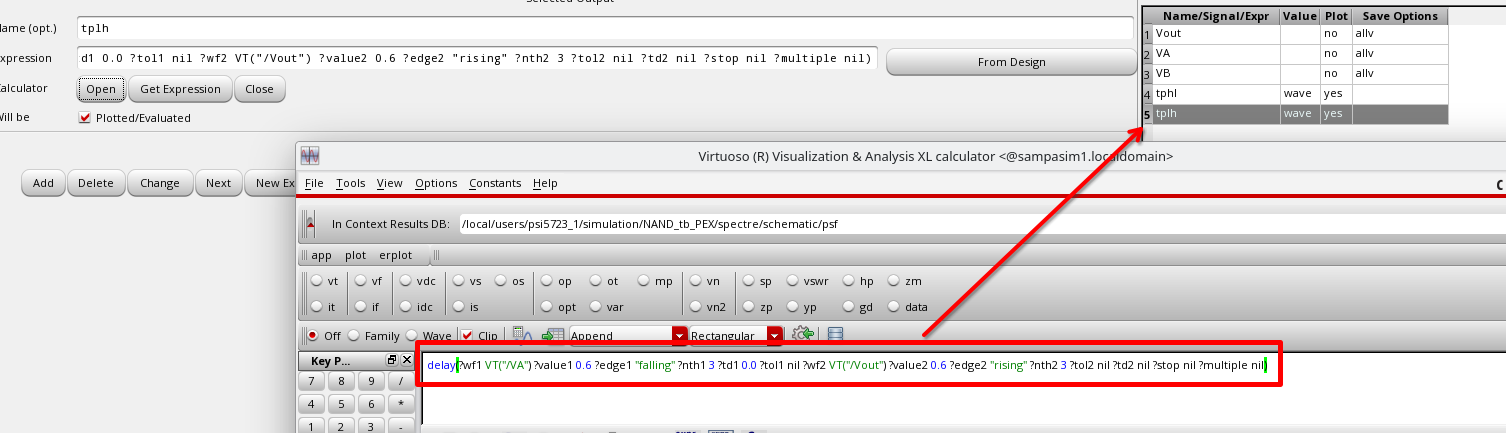
\includegraphics[width=\linewidth]{imagens_lista2_NAND/NAND_tskew_tpLH.png}
    \caption{Expressão \texttt{tplh}: terceira descida de \texttt{/VA} e terceira subida de \texttt{/Vout}, medidas em $600\,\mathrm{mV}$.}
    \label{fig:nand-skew-expr-lh}
\end{figure}

\begin{figure}[!htbp]
    \centering
    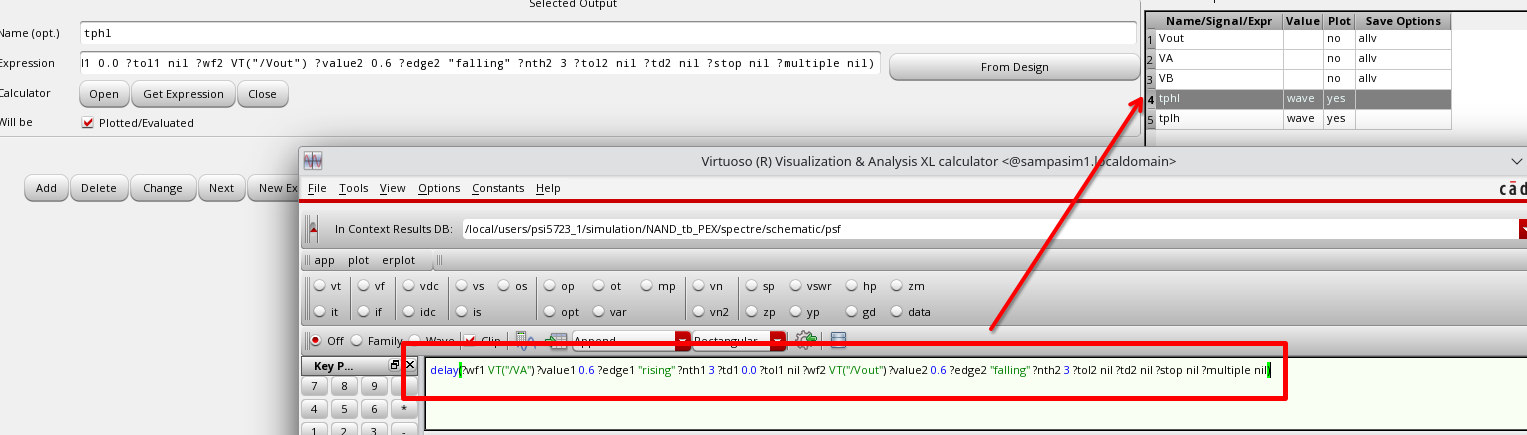
\includegraphics[width=\linewidth]{imagens_lista2_NAND/NAND_tskew_tpHL.png}
    \caption{Expressão \texttt{tphl}: terceira subida de \texttt{/VA} e terceira descida de \texttt{/Vout}, medidas em $600\,\mathrm{mV}$.}
    \label{fig:nand-skew-expr-hl}
\end{figure}

\begin{table}[!htbp]
    \centering
    \caption{Referências e índices de cruzamento usados nas expressões da NAND.}
    \label{tab:nand-skew-medicao}
    \begin{tabular}{lccc}
        \hline
        Expressão & Referência: $A$ & Resposta: $S$ & Limiar\\
        \hline
        \texttt{tplh} & 3ª descida & 3ª subida & $0{,}6\,\mathrm{V}$\\
        \texttt{tphl} & 3ª subida & 3ª descida & $0{,}6\,\mathrm{V}$\\
        \hline
    \end{tabular}
\end{table}

Os intervalos medidos são, portanto,
\begin{align}
    t_{pLH,A} &= t_{S,\uparrow}(50\%)-t_{A,\downarrow}(50\%),\\
    t_{pHL,A} &= t_{S,\downarrow}(50\%)-t_{A,\uparrow}(50\%).
\end{align}

\subsection{Curvas de atraso e extremos}

A Figura~\ref{fig:nand-skew-curvas} apresenta os atrasos em função do skew. A curva vermelha corresponde a $t_{pHL,A}$ e a amarela a $t_{pLH,A}$; os dois eixos estão em picossegundos. Para skew negativo, o atraso de descida fica próximo de $40$ a $44\,\mathrm{ps}$, enquanto o intervalo de subida diminui até assumir valores negativos. Para skew positivo, o atraso de descida cresce quase linearmente, enquanto o de subida tende a aproximadamente $84\,\mathrm{ps}$.

\begin{figure}[!htbp]
    \centering
    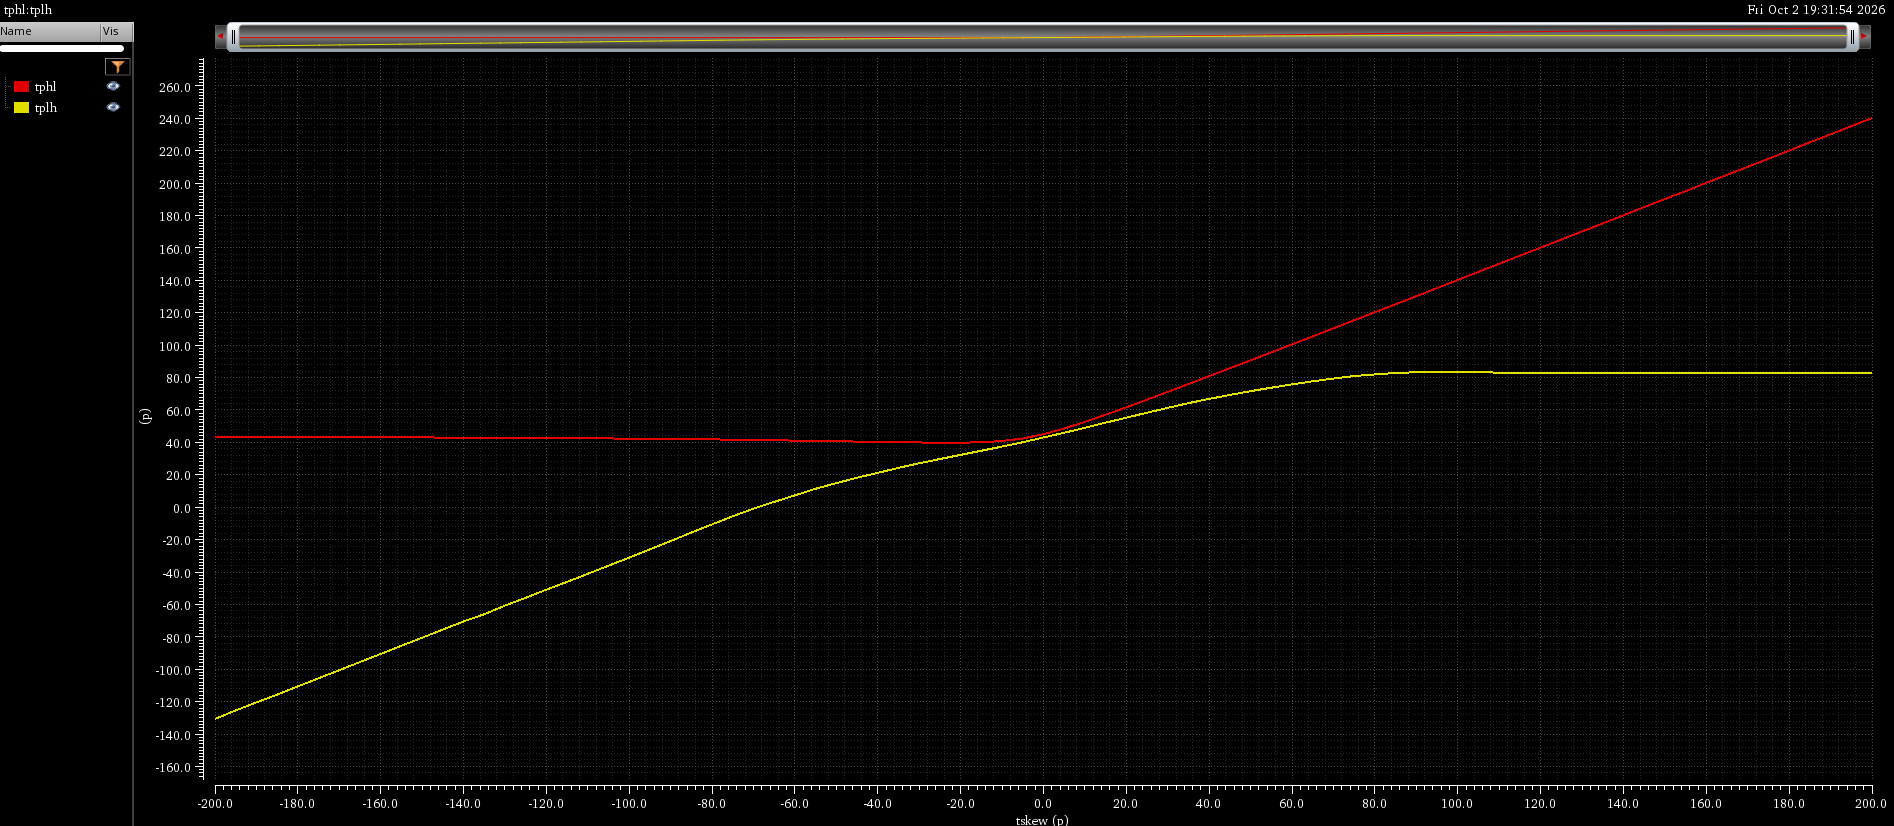
\includegraphics[trim=100bp 0bp 0bp 36bp,clip,width=\linewidth]{imagens_lista2_NAND/NAND_tskew_dealy_seewp.png}
    \caption{Varredura dos atrasos da NAND: $t_{pHL,A}$ em vermelho e $t_{pLH,A}$ em amarelo. Recorte da captura fornecida para ampliar os eixos, sem alteração das curvas.}
    \label{fig:nand-skew-curvas}
\end{figure}

\begin{table}[!htbp]
    \centering
    \caption{Extremos medidos para a porta NAND}
    \label{tab:nand-skew-extremos}
    \begin{tabular}{lcc}
        \hline
        Grandeza & Mínimo & Máximo\\
        \hline
        $t_{pLH,A}$ & $\approx-130\,\mathrm{ps}$
                    & $\approx84\,\mathrm{ps}$ \\
        $t_{pHL,A}$ & $\approx40\,\mathrm{ps}$
                    & $\approx240\,\mathrm{ps}$ \\
        \hline
    \end{tabular}
\end{table}

\section{Atrasos com aplicação de skew para porta NOR}

\subsection{Circuito de teste e aplicação do skew}

Assim como para a porta NAND, nosso ponto de partida foi a implementação da porta NOR na lista 1, onde realizamos o layout, DRC, LVS e extração de capacitâncias parasitas. Esse modelo final foi o que utilizamos no circuito de teste, mostrado na Figura \ref{fig:nor-skew-config}, para os experimentos que vamos detalhar na sequência. Conforme estabelecemos na lista 1, a entrada $A$ controla o PMOS mais próximo de $V_{DD}$, enquanto $B$ controla o PMOS mais próximo da saída. Essa ordem é relevante porque o estado do nó interno entre os PMOS depende de qual entrada comuta primeiro.

\begin{figure}[!htbp]
    \centering
    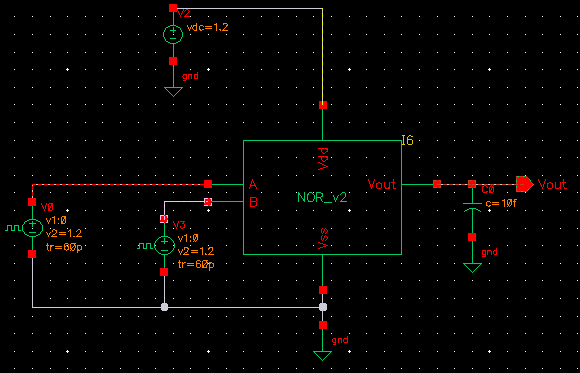
\includegraphics[width=0.65\linewidth]{imagens_lista2_NOR/circuito_NOR.PNG}
    \caption{Circuito de teste da NOR para a análise de skew, com alimentação de $1{,}2\,\mathrm{V}$ e carga de $10\,\mathrm{fF}$.}
    \label{fig:nor-skew-circuito}
\end{figure}

Seguimos o mesmo procedimento utilizado para as medidas com a porta NAND. Como mostrado na Figura~\ref{fig:nor-skew-fontes}, As fontes da  fornecem pulsos entre $0$ e $1{,}2\,\mathrm{V}$, com período de $1\,\mathrm{ns}$, largura de pulso de $200\,\mathrm{ps}$ e rampas de subida e de descida de $60\,\mathrm{ps}$, com largura de pulso de $200\,\mathrm{ps}$. O atraso da fonte $A$ é definido por \texttt{tstart}, enquanto o da fonte $B$ é \texttt{tstart + tskew}. Assim,
\begin{equation}
    t_{\mathrm{skew}} = t_B - t_A.
\end{equation}

\begin{figure}[!htbp]
    \centering
    \begin{minipage}[t]{0.47\linewidth}
        \centering
        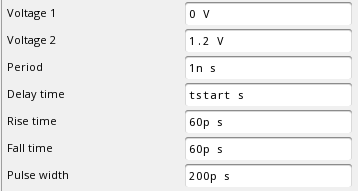
\includegraphics[width=\linewidth]{imagens_lista2_NOR/fonteA.PNG}
        \par\small (a) Fonte da entrada $A$.
    \end{minipage}\hfill
    \begin{minipage}[t]{0.47\linewidth}
        \centering
        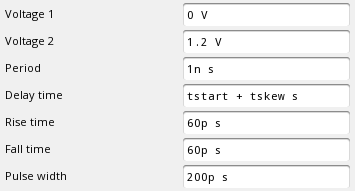
\includegraphics[width=\linewidth]{imagens_lista2_NOR/fonteB.PNG}
        \par\small (b) Fonte da entrada $B$.
    \end{minipage}
    \caption{Configuração das fontes pulsadas. O skew é introduzido exclusivamente no atraso da fonte $B$.}
    \label{fig:nor-skew-fontes}
\end{figure}

A Figura~\ref{fig:nor-skew-ade} documenta a análise transitória de $0$ a $5\,\mathrm{ns}$ e a seleção das entradas, da saída e das expressões \texttt{tpLH} e \texttt{tpHL}. A configuração da ferramenta \textit{Parametric Analysis}, mostrada na Figura~\ref{fig:nor-skew-varredura}, mostra o intervalo de $-200$ a $+200\,\mathrm{ps}$, com incremento de $5\,\mathrm{ps}$, totalizando 81 pontos.

\begin{figure}[!htbp]
    \centering
    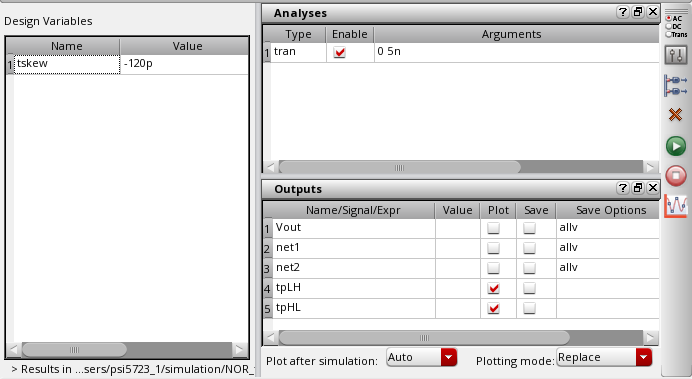
\includegraphics[width=0.90\linewidth]{imagens_lista2_NOR/ADE_setup.PNG}
    \caption{Configuração da análise transitória e das grandezas observadas no ADE.}
    \label{fig:nor-skew-ade}
\end{figure}

\begin{figure}[!htbp]
    \centering
    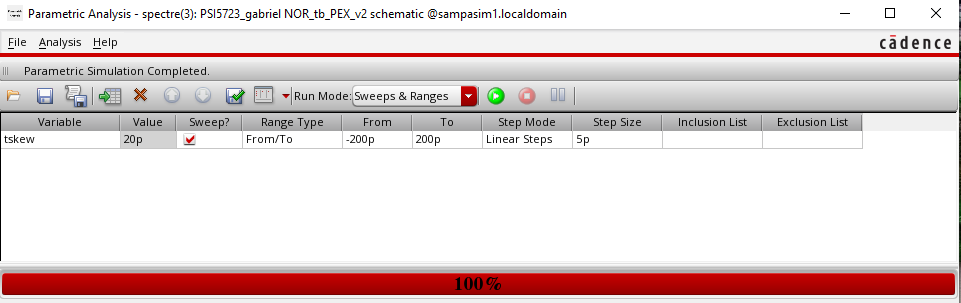
\includegraphics[width=\linewidth]{imagens_lista2_NOR/ParametricAnalysis_Sweep.PNG}
    \caption{Varredura de \texttt{tskew} entre $-200$ e $+200\,\mathrm{ps}$, em passos de $5\,\mathrm{ps}$.}
    \label{fig:nor-skew-varredura}
\end{figure}

\subsection{Critério de medição e índices das bordas}

Novamente, os atrasos foram medidos entre os cruzamentos da entrada de referência e da saída por $50\%$ da alimentação, isto é, por $0{,}6\,\mathrm{V}$. As Figuras~\ref{fig:nor-skew-expr-tplh} e~\ref{fig:nor-skew-expr-tphl} mostram as expressões configuradas na calculadora de expressões do Virtuoso.

Em ambos os casos, a entrada de referência é \texttt{/net1}, correspondente a $A$, e foi selecionada a terceira ocorrência de cada borda, evitando o primeiro ciclo da simulação.

\begin{figure}[!htbp]
    \centering
    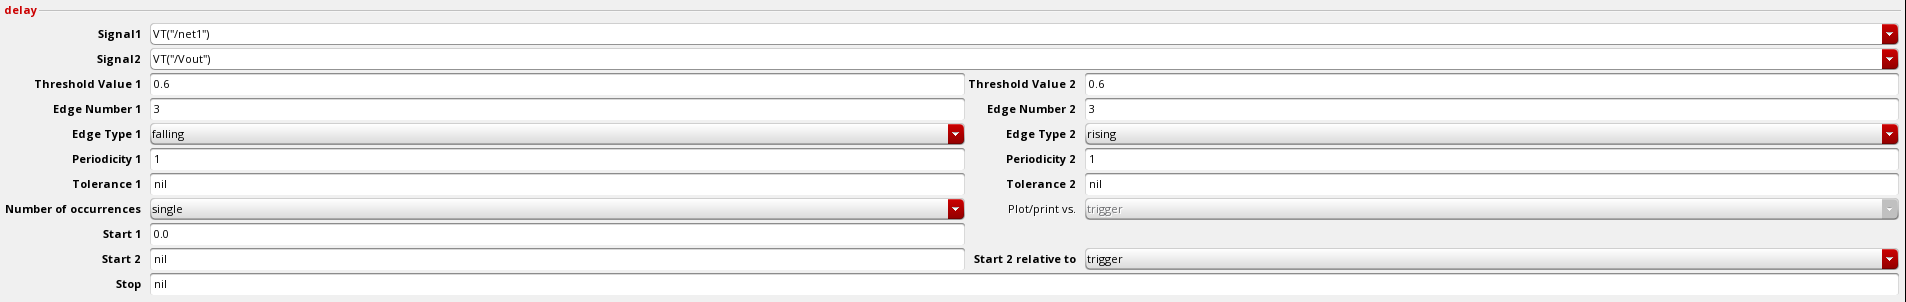
\includegraphics[width=\linewidth]{imagens_lista2_NOR/tpLH_expression.PNG}
    \caption{Expressão utilizada para $t_{pLH}$: diferença entre a terceira borda de descida de $A$ e a terceira borda de subida da saída, ambas em $600\,\mathrm{mV}$.}
    \label{fig:nor-skew-expr-tplh}
\end{figure}

\begin{figure}[!htbp]
    \centering
    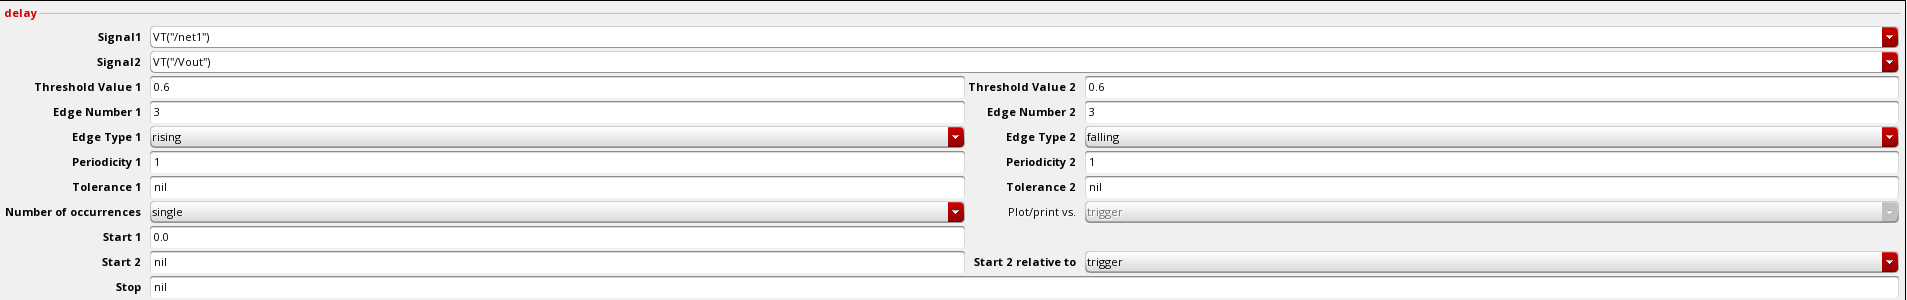
\includegraphics[width=\linewidth]{imagens_lista2_NOR/tpHL_expression.PNG}
    \caption{Expressão utilizada para $t_{pHL}$: diferença entre a terceira borda de subida de $A$ e a terceira borda de descida da saída, ambas em $600\,\mathrm{mV}$.}
    \label{fig:nor-skew-expr-tphl}
\end{figure}

Assim, as grandezas apresentadas pelo ADE são
\begin{align}
    t_{pLH,A} &= t_{S,\uparrow}(0{,}6\,\mathrm{V})
                 -t_{A,\downarrow}(0{,}6\,\mathrm{V}), \\
    t_{pHL,A} &= t_{S,\downarrow}(0{,}6\,\mathrm{V})
                 -t_{A,\uparrow}(0{,}6\,\mathrm{V}).
\end{align}

Como exemplo, a Figura~\ref{fig:nor-skew-transitorio} apresenta as formas de onda disponíveis para $t_{\mathrm{skew}}=+20\,\mathrm{ps}$. Os sinais \texttt{/net1} e \texttt{/net2} correspondem, respectivamente, a $A$ e $B$.

\begin{figure}[!htbp]
    \centering
    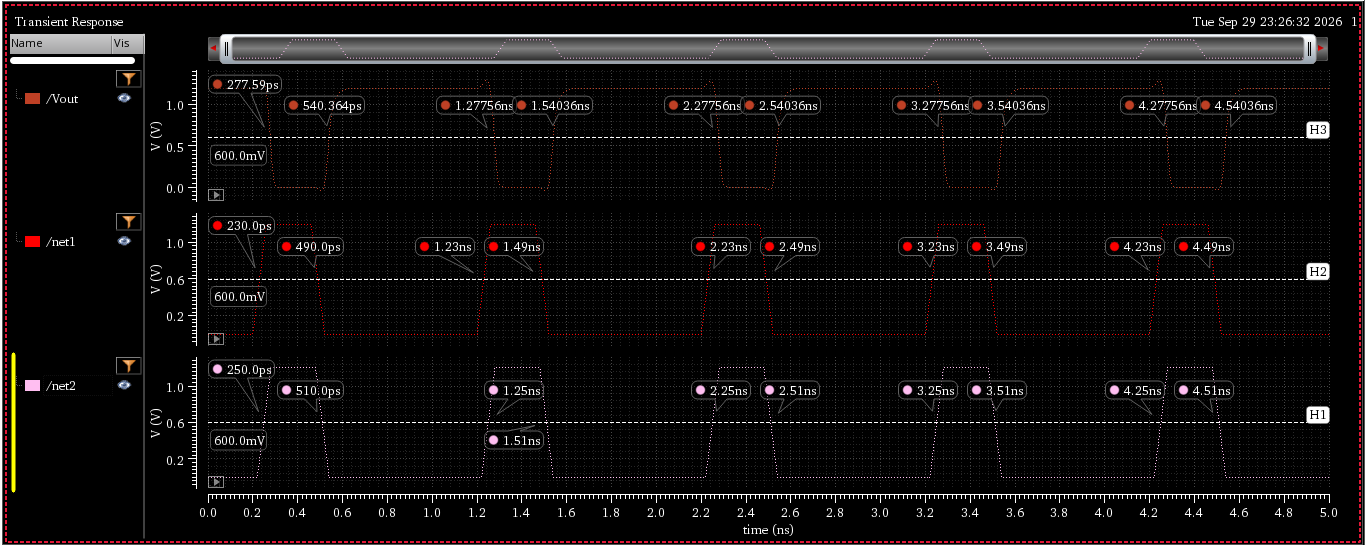
\includegraphics[width=\linewidth]{imagens_lista2_NOR/transient_skew20p.PNG}
    \caption{Formas de onda da saída, de $A$ e de $B$ para $t_{\mathrm{skew}}=+20\,\mathrm{ps}$, com marcadores no nível de $600\,\mathrm{mV}$.}
    \label{fig:nor-skew-transitorio}
\end{figure}

No terceiro ciclo, os cruzamentos de subida das entradas ocorrem em $2{,}230\,\mathrm{ns}$ e $2{,}250\,\mathrm{ns}$, enquanto os cruzamentos de descida ocorrem em $2{,}490\,\mathrm{ns}$ e $2{,}510\,\mathrm{ns}$.

Nesse ciclo, a saída cruza $600\,\mathrm{mV}$ durante a descida em $2{,}27759\,\mathrm{ns}$ e durante a subida em $2{,}54036\,\mathrm{ns}$. Portanto,
\begin{align}
    t_{pHL,A}(+20\,\mathrm{ps})
        &= (2{,}27759-2{,}23000)\,\mathrm{ns}
         =47{,}59\,\mathrm{ps}, \\
    t_{pLH,A}(+20\,\mathrm{ps})
        &= (2{,}54036-2{,}49000)\,\mathrm{ns}
         =50{,}36\,\mathrm{ps}.
\end{align}

\subsection{Curvas de atraso e extremos}

A Figura~\ref{fig:nor-skew-curvas} apresenta $t_{pLH,A}$ e $t_{pHL,A}$ em função de $t_{\mathrm{skew}}$. A escala horizontal está em picossegundos, assim como a escala vertical indicada por \texttt{(p)}. Os valores extremos da Tabela~\ref{tab:nor-skew-extremos} foram estimados diretamente do gráfico na figura.

\begin{figure}[!htbp]
    \centering
    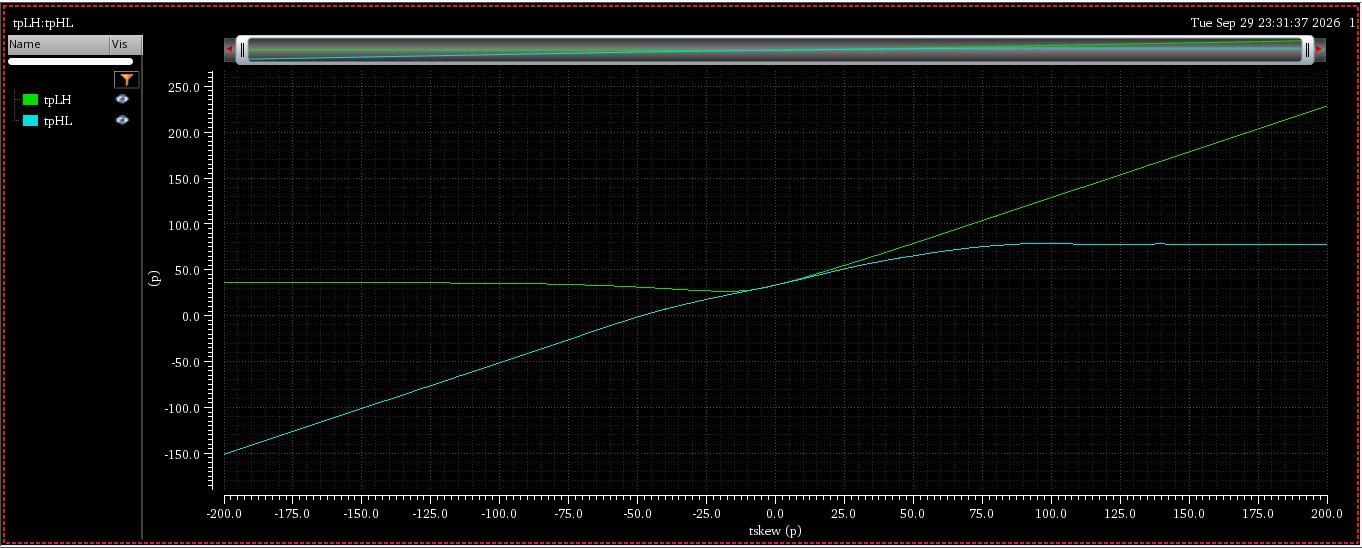
\includegraphics[width=\linewidth]{imagens_lista2_NOR/plot_PropagationDelays_NOR.PNG}
    \caption{Atrasos de propagação da NOR em função do skew: $t_{pLH,A}$ em verde e $t_{pHL,A}$ em ciano.}
    \label{fig:nor-skew-curvas}
\end{figure}

\begin{table}[!htbp]
    \centering
    \caption{Extremos medidos para a porta NAND}
    \label{tab:nor-skew-extremos}
    \begin{tabular}{lcc}
        \hline
        Grandeza & Mínimo & Máximo \\
        \hline
        $t_{pLH,A}$ & $\approx27\,\mathrm{ps}$
                    & $\approx230\,\mathrm{ps}$ \\
        $t_{pHL,A}$ & $\approx-150\,\mathrm{ps}$
                    & $\approx80\,\mathrm{ps}$ \\
        \hline
    \end{tabular}
\end{table}

\section{Análise dos resultados obtidos}

As duas portas apresentam a tendência esperada para entradas deslocadas no tempo. Na NAND, a saída desce após a última entrada subir e sobe após a primeira entrada descer. Na NOR, ocorre o comportamento complementar: a saída desce após a primeira entrada subir e sobe após a última entrada descer. Essa diferença explica por que o ramo que cresce aproximadamente com o skew positivo é $t_{pHL,A}$ na NAND e $t_{pLH,A}$ na NOR.

Há também uma contribuição física além do deslocamento temporal. Na NAND, a comutação simultânea das entradas permite que os dois PMOS carreguem a saída em paralelo; com entradas separadas, a carga começa por apenas um PMOS, justificando o aumento do atraso de subida em relação à região de skew nulo. Como $A$ controla o NMOS inferior, sua subida antecipada pode descarregar o nó interno antes de o NMOS superior ligar. Na NOR, a descarga simultânea se beneficia dos dois NMOS em paralelo, enquanto uma entrada isolada inicia a descarga por apenas um deles. Na rede PMOS em série, $A$ antecipado pode pré-carregar o nó interno, enquanto $B$ antecipado o conecta à saída ainda baixa.

O estado desses nós e a sobreposição das rampas ajudam a explicar a assimetria entre skews positivos e negativos e os pequenos mínimos próximos de zero. Concluímos que as curvas são coerentes com as funções NAND e NOR. Os extremos são fortemente influenciados pelo skew, enquanto as diferenças de comportamento nos dois lados da curva refletem a associação série/paralelo, a ordem das entradas e o estado dos nós internos.

A Tabela~\ref{tab:skew-comparacao-final} reúne os extremos das Tabelas~\ref{tab:nand-skew-extremos} e~\ref{tab:nor-skew-extremos}, se tratam de valores aproximados extraídos dos gráficos nas imagens.

\begin{table}[!htbp]
    \centering
    \caption{Comparação dos extremos dos intervalos referenciados a $A$. Valores em ps; a amplitude é máximo menos mínimo. A razão não é usada para extremos de sinais opostos.}
    \label{tab:skew-comparacao-final}
    \begin{tabular}{llcccc}
        \hline
        Porta & Grandeza & Mínimo & Máximo & $\Delta$ \\
        \hline
        NAND & $t_{pLH,A}$ & $-130$ & $84$  & $214$ \\
        NAND & $t_{pHL,A}$ & $40$   & $240$ & $200$ \\
        NOR  & $t_{pLH,A}$ & $27$   & $230$ & $203$ \\
        NOR  & $t_{pHL,A}$ & $-150$ & $80$  & $230$ \\
        \hline
    \end{tabular}
\end{table}

\end{document}